\documentclass[11pt]{buthesis}

\usepackage[T1]{fontenc}
\usepackage[utf8]{inputenc}
\usepackage{amsmath}
\usepackage{array}
\usepackage{booktabs}
\usepackage{enumitem}
\usepackage{microtype}
\usepackage[section]{placeins}
\usepackage{pgfplots}
\usepackage{tikz}
\usepackage{url}

\usetikzlibrary{arrows.meta,positioning}
\usepgfplotslibrary{groupplots}
\pgfplotsset{compat=1.18}
\numberwithin{equation}{chapter}
\DeclareMathOperator*{\argmin}{arg\,min}
\DeclareMathOperator*{\argmax}{arg\,max}

\title{Capability-Bounded Code Evolution with Large Language Models\\
A Cross-Family Study of Adaptive Heuristic Search}
\author{Fabio Cozzuto}
\dept{Computer Science}
\degree{Master of Science}
\submitdate{June 2026}
\copyrightyear{2026}

\begin{document}

\beforepreface

\prefacesection{Abstract}
Large language models can now write executable code, repair programs, and participate in
evaluator-guided search loops. These capabilities raise a concrete research question for
computer science: can a language-model-driven code-evolution loop produce useful heuristic
programs beyond one-shot generation, and under what conditions do apparent improvements
reflect genuine adaptation rather than extra search budget or benchmark idiosyncrasies? This
dissertation studies that question through a unified experimental framework in which models
iteratively propose deterministic Python heuristics, receive structured feedback from
task-specific validators, and are compared under replicated conditions on increasingly realistic
problem families. The framework begins with simple adversarial games, then moves to benchmark
combinatorial optimization tasks based on symmetric and asymmetric traveling salesperson
problems and capacitated vehicle routing. Across these settings, the dissertation evaluates
replay-aware memory mechanisms, modular operator discovery, adaptive heuristic portfolios, and
budget-matched controls intended to separate genuine evolutionary effects from additional
sampling. The evidence supports a capability-bounded account rather than broad
algorithm-discovery dominance. The code-evolution loop reliably produces diverse executable
heuristic variants and can preserve useful refinements when the benchmark leaves reachable
heuristic headroom, but its apparent gains are strongly constrained by validator pressure,
baseline strength, and task-specific interaction structure. In the final budget-controlled
factorial analysis, replay-specific mechanisms do not show robust added value over
budget-matched independent search. The dissertation contributes a measurement framework for
studying when LLM-guided code evolution adapts, when it churns, and which failure modes recur
across domains.

\prefacesection{Acknowledgments}
The author thanks Dr. Russell Butler for his supervision, guidance, and feedback throughout this
research.

\afterpreface

\chapter{Introduction}
\label{chap:introduction}
\chapterrunning{introduction}

The design of effective heuristics remains one of the central practical problems in computer
science. Many computational tasks of scientific and industrial importance, including routing,
scheduling, and resource allocation, are too expensive to solve exactly at the scales demanded by
real applications. As a result, practitioners routinely rely on hand-crafted heuristics,
metaheuristics, or solver portfolios whose quality depends heavily on human insight, empirical
tuning, and domain knowledge \cite{rice1976,bengio2021mlco,burke2013,dokeroglu2024}. The
question of how to automate some portion of this design process has therefore persisted across
operations research, machine learning, and evolutionary computation for decades.

Recent progress in large language models (LLMs) changes the form of this question. Modern code
models can synthesize non-trivial executable programs from natural-language specifications, solve
benchmark programming tasks, and improve performance through repeated sampling and automated
testing \cite{chen2021codex,austin2021program,li2022alphacode,zan2023nl2code,jiang2024codesurvey,jain2024livecodebench}.
More importantly for optimization, these models can be embedded inside outer loops that evaluate
candidate programs, retain strong variants, and request improved descendants. Systems such as
AlphaDev and FunSearch show that evaluator-guided search can go beyond naive one-shot completion
when the problem admits fast verification and a suitably structured search space
\cite{mankowitz2023alphadev,romeraparedes2024funsearch}. At the same time, early work on LLMs as
evolutionary optimizers suggests both promise and sharp scale limitations, especially when the
search is applied to combinatorial optimization rather than small synthetic benchmarks
\cite{liu2023lmea,daros2025llmco}.

These developments motivate the present dissertation. The central question is whether repeated
proposal, evaluation, and revision can improve executable heuristics in a way that survives
stronger benchmarks and stronger baselines. That question also requires tighter controls on
interpretation. Apparent gains may
reflect useful adaptation, but they may also reflect benchmark headroom, weak baselines, or prompt
sequences that generate many variants without preserving a real improvement. The dissertation
examines iterative code evolution as an empirical object that must be measured across more than one
family and judged by held-out results rather than by isolated successful artifacts.

\section{Problem Statement}
\label{sec:intro-problem}

This dissertation studies LLM-guided code evolution as a \emph{measurable adaptive search loop}
rather than as a general claim of autonomous algorithm invention. The framework considered here is
simple by design. A model receives a constrained programming interface and task feedback, proposes
a deterministic Python heuristic, and then receives structured information about the heuristic's
behaviour and performance. The loop repeats over many epochs, storing code variants, validator
signals, and archive summaries that can be replayed into later prompts. The scientific objective
is to determine when such a loop adapts in a useful way and when it merely produces syntactically
different but functionally unimportant variants.

The dissertation addresses the following research question:

\begin{quote}
Under what conditions does an LLM-guided code-evolution loop generate useful heuristic adaptation,
and when are apparent gains better explained by search budget, benchmark headroom, validator
pressure, or baseline strength?
\end{quote}

This broad question is instantiated through several narrower empirical questions distributed
across the dissertation:

\begin{enumerate}[leftmargin=2em]
\item Do replay-aware memory mechanisms improve held-out performance relative to no replay, random
replay, and other replay-selection rules?
\item Does the answer remain stable when the environment shifts from toy adversarial games to
standard benchmark optimization families such as TSPLIB and CVRPLIB?
\item Can the search loop discover reusable heuristic components or adaptive controllers, rather
than only full-program variants tied to a single scaffold?
\item How strongly do validator pressure, baseline strength, and benchmark headroom limit the gains
that the loop can realize on held-out instances?
\end{enumerate}

\section{Research Objectives}
\label{sec:intro-objectives}

The project is organized around four concrete objectives.

\begin{enumerate}[leftmargin=2em]
\item To formalize LLM-guided code evolution as a controlled experimental pipeline rather than an
anecdotal prompt-engineering exercise.
\item To evaluate the pipeline on benchmark families whose structure and baseline difficulty differ
materially, namely simple games, TSP, ATSP, and CVRP.
\item To distinguish family-specific replay effects from more general claims about memory, broader
search, or benchmark-specific headroom.
\item To produce a conservative account of the present capabilities and limits of executable
heuristic evolution by LLMs, including null results and bounded wins.
\end{enumerate}

\section{Working Hypotheses}
\label{sec:intro-hypotheses}

The hypotheses below state the principal empirical claims examined in this dissertation. They are
framed to distinguish mechanism-specific effects from broader effects due to search budget,
benchmark structure, and baseline strength.

\begin{enumerate}[leftmargin=2em]
\item \textbf{H1: Adaptive search under validator feedback.} When a benchmark family contains
reachable heuristic headroom and the interface remains executable under repeated sampling, an
iterative LLM-guided loop will generate non-trivial behavioural diversity and occasionally improve
held-out quality over one-shot sampling.
\item \textbf{H2: Replay must justify its added machinery.} A replay or archive mechanism should be
credited only when it improves held-out performance relative to simpler controls or alternative
replay rules evaluated under the same protocol.
\item \textbf{H3: Gains shrink under stronger evaluators.} Apparent advantages of evolved code
should weaken as validator pressure rises, feasibility constraints tighten, and classical baselines
consume more of the available benchmark headroom.
\item \textbf{H4: Transfer is partial rather than universal.} Search components discovered on one
family may transfer across related problems, but the strength of that transfer should depend on the
interaction structure of the target domain rather than on a task-agnostic notion of ``general
algorithmic intelligence.''
\end{enumerate}

These hypotheses permit negative or mixed outcomes. Under controlled evaluation, null results are
informative because they help separate genuine mechanism effects from artefacts of sampling budget
or benchmark choice.

\section{Formal Setup and Notation}
\label{sec:intro-formal-setup}

The dissertation treats heuristic search as a problem of learning or discovering \emph{programs}
that map benchmark instances to feasible solutions. Let $\mathcal{X}$ denote a family of problem
instances, let $\Omega(x)$ denote the feasible solution set for instance $x \in \mathcal{X}$, and
let $f(\cdot;x)$ denote a minimization objective on $\Omega(x)$.

\begin{definition}
A \emph{benchmark optimization family} is a triple
$\mathcal{F} = (\mathcal{X}, \Omega, f)$ consisting of an instance distribution or benchmark set
$\mathcal{X}$, a feasibility map $\Omega$, and an objective function $f$ to be minimized.
\end{definition}

\begin{definition}
A \emph{deterministic heuristic program} for $\mathcal{F}$ is an executable mapping
$h : \mathcal{X} \to \Omega(x) \cup \{\bot\}$ that returns either a feasible solution or a
detectable failure symbol $\bot$ under a fixed interface and resource budget.
\end{definition}

This definition covers the constructive game agents of the early phases, the TSP and ATSP
tour-construction heuristics of the routing phases, and the bounded CVRP solvers evolved in the
later real-world experiments. The relevant distinction is whether a program yields a measurable
objective value under controlled execution.

For any evaluation panel $\mathcal{D} \subseteq \mathcal{X}$, the empirical quality of a heuristic
program is summarized by an aggregate metric
\begin{equation}
J_{\mathcal{D}}(h) = \frac{1}{|\mathcal{D}|}\sum_{x \in \mathcal{D}} \operatorname{gap}(h,x),
\label{eq:intro-aggregate-gap}
\end{equation}
where lower values are better and the instance-level gap is defined, whenever a reference cost
$f^{\star}(x)$ is available, by
\begin{equation}
\operatorname{gap}(h,x) =
\frac{f(h(x);x)-f^{\star}(x)}{f^{\star}(x)}.
\label{eq:intro-relative-gap}
\end{equation}
For feasibility-constrained settings such as CVRP, the implementation can replace $f$ by a
penalized objective $\tilde{f}$ that incorporates route-capacity or constraint violations. The
form of \eqref{eq:intro-relative-gap} is standard in routing benchmarks because it allows
comparisons across instances of different scales.

\begin{definition}
An \emph{LLM-guided code-evolution loop} is an iterative process over a program space
$\mathcal{H}$ with prompt state $p_t$, archive state $\mathcal{A}_t$, and evaluator $E$, such that
\begin{align}
h_t &\sim q_{\phi}(\cdot \mid p_t), \label{eq:intro-sampling}\\
r_t &= E(h_t; \mathcal{D}_{\mathrm{train}}), \label{eq:intro-evaluation}\\
\mathcal{A}_t &= U(\mathcal{A}_{t-1}, h_t, r_t), \label{eq:intro-archive-update}\\
p_{t+1} &= C(\mathcal{T}, \mathcal{A}_t, r_t), \label{eq:intro-prompt-update}
\end{align}
where $q_{\phi}$ is the model-conditioned program generator, $U$ is the archive update rule, and
$C$ constructs the next prompt from the task specification $\mathcal{T}$ and archived evidence.
\end{definition}

Equations \eqref{eq:intro-sampling}--\eqref{eq:intro-prompt-update} make the research claim
precise: replay is not a vague intuition, but a specific modification of the archive state
$\mathcal{A}_t$ and prompt-construction operator $C$. A replay mechanism has independent value only
if it improves final held-out performance relative to an explicit control condition. One generic
comparison can be expressed as
\begin{equation}
\Delta_{\mathrm{replay}} =
J_{\mathcal{D}_{\mathrm{test}}}\!\left(h^{\mathrm{replay}}\right) -
J_{\mathcal{D}_{\mathrm{test}}}\!\left(h^{\mathrm{control}}\right),
\label{eq:intro-replay-delta}
\end{equation}
where a robustly negative value of $\Delta_{\mathrm{replay}}$ would support a replay-specific
advantage on a lower-is-better metric.

To separate meaningful behavioural diversity from mere lexical change, the loop also tracks
novelty-like signals. A generic archive-relative novelty score can be written as
\begin{equation}
\nu(h_t,\mathcal{A}_{t-1}) =
1 - \max_{h \in \mathcal{A}_{t-1}} \operatorname{sim}(h_t,h),
\label{eq:intro-novelty}
\end{equation}
where $\operatorname{sim}$ is a code- or behaviour-level similarity measure. No single novelty
metric is assumed to be canonical; novelty is treated as a diagnostic that must be interpreted
jointly with validator outcomes and held-out quality.

\begin{table}[t]
\centering
\small
\setlength{\tabcolsep}{3pt}
\begin{tabular}{>{\raggedright\arraybackslash}p{0.95in} >{\raggedright\arraybackslash}p{3.85in}}
\toprule
Symbol & Meaning \\
\midrule
$\mathcal{X}$ & benchmark family or instance space \\
$x \in \mathcal{X}$ & a specific optimization instance \\
$\Omega(x)$ & feasible solution set for instance $x$ \\
$f(\cdot;x)$ & instance-level minimization objective \\
$J_{\mathcal{D}}(h)$ & aggregate evaluation metric of heuristic $h$ on panel $\mathcal{D}$ \\
$\mathcal{H}$ & constrained program space searched by the outer loop \\
$q_{\phi}$ & model-conditioned proposal distribution over candidate programs \\
$\mathcal{A}_t$ & archive or replay state available at iteration $t$ \\
$E$ & validator and scorer used to evaluate a candidate program \\
$\nu(h_t,\mathcal{A}_{t-1})$ & archive-relative novelty diagnostic for candidate $h_t$ \\
\bottomrule
\end{tabular}
\caption[Core notation]{Core notation used throughout the introduction and later methodological chapters.}
\label{tab:intro-notation}
\end{table}

\begin{figure}[t]
\centering
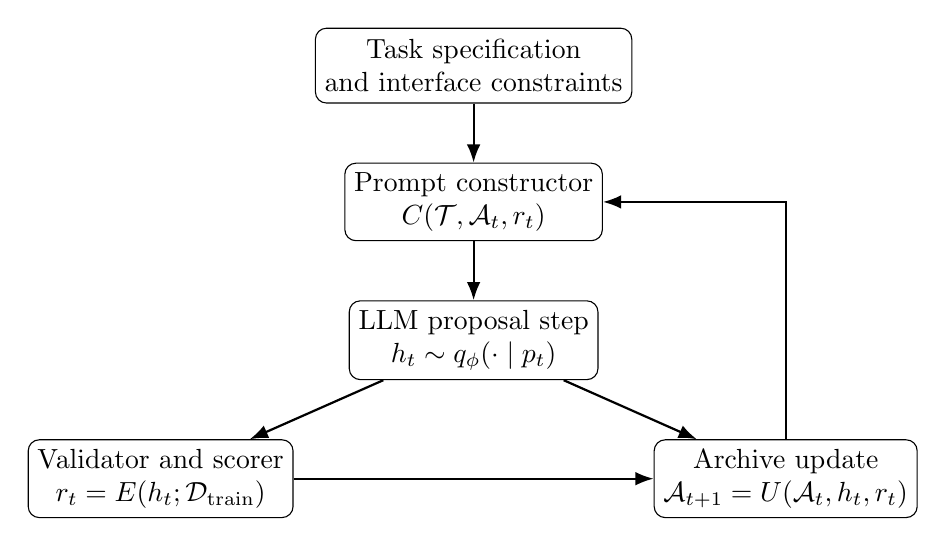
\begin{tikzpicture}[
  node distance=0.75cm and 0.6cm,
  box/.style={draw, rounded corners, align=center, minimum width=3.15cm, minimum height=0.95cm},
  line/.style={-Latex, thick}
]
\node[box] (task) {Task specification\\and interface constraints};
\node[box, below=of task] (prompt) {Prompt constructor\\$C(\mathcal{T}, \mathcal{A}_t, r_t)$};
\node[box, below=of prompt] (model) {LLM proposal step\\$h_t \sim q_{\phi}(\cdot \mid p_t)$};
\node[box, below left=of model, xshift=-0.1cm] (eval) {Validator and scorer\\$r_t = E(h_t;\mathcal{D}_{\mathrm{train}})$};
\node[box, below right=of model, xshift=0.1cm] (archive) {Archive update\\$\mathcal{A}_{t+1}=U(\mathcal{A}_t,h_t,r_t)$};
\draw[line] (task) -- (prompt);
\draw[line] (prompt) -- (model);
\draw[line] (model) -- (eval);
\draw[line] (model) -- (archive);
\draw[line] (eval) -- (archive);
\draw[line] (archive.north) |- (prompt.east);
\end{tikzpicture}
\caption[Conceptual code-evolution loop]{Conceptual structure of the LLM-guided code-evolution loop studied in this dissertation.
The central question is whether the closed loop between archive, validator, and proposal model
produces reliable adaptation under controlled protocols.}
\label{fig:intro-loop}
\end{figure}

\section{Why This Question Matters}
\label{sec:intro-motivation}

The practical motivation follows directly from the role of heuristics in large-scale optimization.
If language models can participate productively in heuristic search, then they could become useful
assistants for constructing bounded optimization procedures in domains where exact methods are too
slow and hand-designed heuristics are expensive to develop. The scientific motivation is subtler.
Recent work on LLM-based scientific and algorithmic discovery has highlighted competitive
programming performance, small algorithmic improvements, and evaluator-guided discoveries in
specialized settings
\cite{li2022alphacode,mankowitz2023alphadev,romeraparedes2024funsearch}. Those results are
important, but they do not by themselves establish a general understanding of when an LLM-driven
search loop should work, when it should fail, and which controls are necessary to distinguish true
adaptation from a larger sampling budget.

This issue is especially important in stochastic learning systems, where optimistic conclusions can
be driven by best-run anecdotes, fragile benchmarks, or insufficient controls. Empirical machine
learning has already seen the cost of such under-specified reporting, particularly in reinforcement
learning, where replicated evaluation, uncertainty-aware summaries, and strong baselines are now
widely recognized as necessary for credible claims \cite{henderson2018drltm,agarwal2021precipice}.
The same discipline is needed here. A dissertation on LLM-guided heuristic evolution should not
only report positive cases. It should also identify limits, null results, and failure mechanisms.

\section{Dissertation Scope}
\label{sec:intro-scope}

The work reported here begins with simple adversarial games and then moves to increasingly
realistic combinatorial optimization families. This progression is deliberate. The initial game
environments provide a cheap setting in which iterative adaptation, curriculum effects, replay,
and behavioural diversity can be observed directly. Later phases retain the same basic
code-evolution machinery but replace the toy environment with benchmark-driven tasks whose solution
quality can be evaluated against established references and classical heuristics. In particular,
the dissertation studies:

\begin{enumerate}[leftmargin=2em]
\item adversarial code evolution in simple two-player games;
\item replay-aware heuristic evolution on symmetric TSPLIB traveling salesperson benchmarks;
\item transfer of the same design ideas to asymmetric TSPLIB ATSP and CVRPLIB CVRP families;
\item modular operator discovery and adaptive heuristic portfolio control on TSP;
\item bounded whole-solver evolution on real-world CVRPLIB X instances; and
\item a cross-family synthesis of the completed simple-game, TSP, and real-world CVRP evidence,
together with a descriptive direct Codex baseline on bounded CVRP.
\end{enumerate}

\begin{table}[t]
\centering
\scriptsize
\setlength{\tabcolsep}{3pt}
\begin{tabular}{
  >{\raggedright\arraybackslash}p{0.65in}
  >{\raggedright\arraybackslash}p{1.1in}
  >{\raggedright\arraybackslash}p{1.35in}
  >{\raggedright\arraybackslash}p{1.1in}
}
\toprule
Family & Benchmark basis & Evolved artifact & Primary held-out metric \\
\midrule
Simple games & synthetic adversarial environments & deterministic game-playing policy code & win rate / score margin \\
TSP & TSPLIB symmetric routing instances & tour-construction or improvement heuristic code & relative optimality gap \\
ATSP & TSPLIB asymmetric routing instances & transfer-tested heuristic code & relative optimality gap \\
CVRP & CVRPLIB, especially Uchoa X instances & whole solver or route-construction code & penalized gap with feasibility pressure \\
\bottomrule
\end{tabular}
\caption[Problem families and evaluation focus]{Problem families covered by the dissertation and the corresponding evaluation focus.}
\label{tab:intro-families}
\end{table}

The study therefore extends beyond a single TSP setting, but it does not attempt to formulate a
universal theory of automatic algorithm discovery. Its aim is narrower: to develop a unified
framework for studying \emph{capabilities and limits} in LLM-guided code evolution across domains
with different structural demands.

\section{Main Thesis}
\label{sec:intro-main-thesis}

The central thesis of this dissertation is as follows:

\begin{quote}
Across simple games, TSP, ATSP, and real-world CVRP, LLM-guided code evolution can generate
diverse executable heuristic programs and sometimes preserve useful adaptations, but its success is
capability-bounded. In the current evidence, performance depends strongly on validator pressure,
baseline strength, benchmark headroom, and task-specific interaction structure. Replay-specific
mechanisms matter in some settings, but no single replay recipe remains dominant across the
completed benchmark families.
\end{quote}

The completed results support a conservative interpretation. They do not support two stronger
claims: that replay uniformly improves performance, or that iterative LLM search has already
surpassed mature human-designed optimization heuristics in a general sense. Instead, the empirical
record identifies where adaptation occurs, where it fails to transfer, and how meaningful
improvement can be separated from superficial novelty and favorable benchmark conditions.

\section{Research Contributions}
\label{sec:intro-contributions}

The dissertation makes five main contributions.

\begin{enumerate}[leftmargin=2em]
\item It introduces a unified experimental framework for iterative code evolution with archived
feedback, constrained execution, deterministic validators, and report-first research artifacts.
\item It extends the study of replay-aware code evolution from toy adversarial settings to multiple
benchmark optimization families, including symmetric TSP, asymmetric TSP, and capacitated vehicle
routing.
\item It evaluates not only positive search variants but also mechanism-focused alternatives,
including curated failure replay, compression pressure, modular operator evolution, and
portfolio-based selection under strong fixed baselines.
\item It emphasizes replicated, uncertainty-aware, benchmark-based evaluation in the spirit of
careful empirical RL methodology \cite{henderson2018drltm,agarwal2021precipice}.
\item It contributes a conservative cross-family synthesis in which negative and boundary results
are treated as findings, not as failures to be hidden.
\end{enumerate}

\section{Preview of Findings}
\label{sec:intro-preview}

The main empirical findings are mixed but coherent.

First, the game phases show real functional adaptation, but the novelty audit also shows that many
large code changes are mixed or negative rather than uniformly useful. Second, replay can help on
benchmark routing, but not in the simple way initially hypothesized. On symmetric TSP, naive
raw-failure replay is not the strongest mechanism; curation matters more than failure accumulation
alone, and compression does not help the strongest replay arms. Third, the family extensions block
any universal replay claim: ATSP yields only a weak compression-aware signal, while no-replay
remains strongest on the replicated phase-5 CVRP suite. Fourth, the later higher-upside phases act
as strict falsification tests. Modular operator discovery produces genuine rediscovery structure,
yet no operator survives the full validation pipeline. Adaptive portfolio control improves over a
weak one-shot LLM selector, yet does not beat the strongest fixed heuristic or the supervised
selector when oracle headroom is absent on the primary endpoint. Whole-solver evolution on
real-world CVRP stays feasible and improves over weaker bounded baselines, but not over the fixed
Clarke--Wright baseline. Finally, the cross-family synthesis supports a capability-bounded account
in which executable variation is common, but durable gains depend on the target family and on the
strength of the competing baseline.

\begin{figure}[t]
\centering
\begin{tikzpicture}
\begin{groupplot}[
  group style={group size=2 by 1, horizontal sep=1.1cm},
  width=0.40\textwidth,
  height=0.24\textheight,
  ymin=0,
  scaled y ticks=false,
  enlarge x limits=0.18,
  axis line style={black},
  tick style={black},
  ylabel={Lower-is-better gap},
  xtick=data,
  x tick label style={font=\scriptsize, rotate=25, anchor=east},
  yticklabel style={
    font=\footnotesize,
    /pgf/number format/fixed,
    /pgf/number format/precision=2
  },
  every axis title/.style={font=\small},
  title style={at={(0.5,1.03)}, anchor=south},
  point meta=y,
  nodes near coords={\pgfmathprintnumber[fixed,precision=3]{\pgfplotspointmeta}},
  every node near coord/.append style={font=\tiny, anchor=south, yshift=1pt, text=black},
]
\nextgroupplot[
  title={TSP replay suite},
  ymax=0.145,
  symbolic x coords={No replay,Failure,Compression,Random},
]
\addplot+[ybar, draw=black, fill=black!20, bar width=9pt] coordinates {
  (No replay,0.132474)
  (Failure,0.130918)
  (Compression,0.124895)
  (Random,0.104243)
};

\nextgroupplot[
  title={CVRP held-out suite},
  ymax=0.52,
  ylabel={},
  symbolic x coords={CW savings,Evolution,NN,Regret+LS},
]
\addplot+[ybar, draw=black, fill=black!45, bar width=9pt] coordinates {
  (CW savings,0.073766)
  (Evolution,0.182231)
  (NN,0.273435)
  (Regret+LS,0.466391)
};
\end{groupplot}
\end{tikzpicture}
\caption[Representative held-out phase results]{Representative held-out results from completed project phases. Lower is better in both
panels. In the TSP replay suite, random replay achieved the best mean transfer gap among the
replay variants. In the real-world CVRP suite, solver evolution improved over weaker bounded
baselines yet remained behind the fixed Clarke--Wright savings heuristic on the primary endpoint.}
\label{fig:intro-preview-results}
\end{figure}

Overall, these findings support a \emph{capability-and-limits} interpretation. The system is good
enough to warrant serious study, but not strong enough to justify claims of general
algorithm-discovery superiority.

\section{Organization of the Dissertation}
\label{sec:intro-organization}

The remainder of the dissertation is organized as follows. Chapter~\ref{chap:literature-review}
reviews the literature on heuristics and algorithm selection, machine learning for combinatorial
optimization, LLM-based code generation, evaluator-guided algorithm discovery, and curriculum,
replay, and diversity mechanisms. Chapter~\ref{chap:methodology} presents the common experimental
framework, replication discipline, and reporting methodology. Chapter~\ref{chap:simple-games}
reports the adversarial transfer evidence and the manual novelty adjudication. Chapter~
\ref{chap:routing-studies} examines the replicated routing replay and replay-mechanism results
across TSP, ATSP, and CVRP. Chapter~\ref{chap:advanced-phases} presents the operator-discovery,
adaptive-portfolio, and real-world CVRP solver-evolution phases. Chapter~\ref{chap:conclusion}
returns to the main hypotheses, synthesizes the cross-family evidence, and outlines the principal
limitations and future research directions.

\chapter{Literature Review}
\label{chap:literature-review}
\chapterrunning{literature review}

\section{Heuristics, Hyper-Heuristics, and Algorithm Selection}
\label{sec:lit-heuristics}

The practical difficulty of many combinatorial optimization problems has long made heuristic design
an essential part of computer science and operations research. Rice's classic formulation of the
algorithm selection problem cast the issue in its most general form: given a space of instances, a
portfolio of candidate algorithms, and a performance measure, the task is to learn or construct a
mapping from instances to algorithms that performs well in expectation \cite{rice1976}. In modern
notation, if $\mathcal{X}$ is an instance family, $\mathcal{A}$ is a portfolio of algorithms, and
$m(a,x)$ is a lower-is-better performance metric, then the ideal selector is
\begin{equation}
\pi^{\star} \in \argmin_{\pi : \mathcal{X} \to \mathcal{A}}
\mathbb{E}_{x \sim \mathcal{D}}[m(\pi(x),x)].
\label{eq:lit-alg-selection}
\end{equation}
Equation~\eqref{eq:lit-alg-selection} remains foundational because it separates the underlying
optimization problem from the meta-level question of which procedure should be applied to which
instance.

Hyper-heuristics emerged as one prominent response to this meta-level challenge. Rather than
searching directly over candidate solutions, hyper-heuristics search over heuristics or heuristic
components, with the goal of automating heuristic selection, sequencing, or generation
\cite{burke2013,dokeroglu2024}. This shift from solution space to heuristic space is especially
relevant for the present dissertation because the proposed LLM-guided loop also operates primarily
at the level of \emph{programs that produce solutions}, not at the level of solutions themselves.
Recent surveys emphasize that hyper-heuristics now span selection, generation, portfolio, and
configuration settings, and that modern work increasingly integrates machine learning into all four
categories \cite{dokeroglu2024}. The present dissertation belongs to this tradition, with the
difference that the search operator is a language model capable of proposing new executable code
rather than a classical mutation, grammar, or rule-combination mechanism.

Algorithm selection has likewise evolved toward both feature-based and feature-free approaches.
Traditional methods rely on hand-designed instance descriptors, whereas newer methods attempt to
learn directly from raw instance representations \cite{alissa2023}. This distinction becomes
important in later chapters, especially for the adaptive heuristic portfolio experiments, because
it frames a key design choice: should a controller rely on explicit descriptors crafted from domain
knowledge, or can a more generic representation learn the selector implicitly?

\section{Formal Benchmark Problem Definitions}
\label{sec:lit-problems}

The empirical phases of this dissertation are built around standard benchmark optimization
families. A concise formal account is therefore useful before turning to learning-based methods.

\subsection{Symmetric Traveling Salesperson Problem}
\label{sec:lit-tsp}

In the symmetric traveling salesperson problem (TSP), one is given a complete weighted graph
$G = (V,E,w)$ with $w_{ij} = w_{ji} \geq 0$ and seeks a minimum-cost Hamiltonian cycle
\cite{reinelt1991}. Using binary edge-selection variables $x_{ij}$, a standard formulation is
\begin{align}
\min_{x} \quad & \sum_{(i,j)\in E} w_{ij}x_{ij} \label{eq:lit-tsp-obj} \\
\text{s.t.} \quad
& \sum_{j \neq i} x_{ij} = 2, && \forall i \in V, \label{eq:lit-tsp-degree}\\
& \sum_{i,j \in S,\ i<j} x_{ij} \le |S|-1, && \forall S \subset V,\ 2 \le |S| < |V|, \label{eq:lit-tsp-subtour}\\
& x_{ij} \in \{0,1\}, && \forall (i,j)\in E. \label{eq:lit-tsp-binary}
\end{align}
Constraint \eqref{eq:lit-tsp-degree} enforces degree two at every city, while
\eqref{eq:lit-tsp-subtour} removes disconnected subtours. The TSP is NP-hard, which explains why
heuristic methods remain central despite decades of exact and approximate progress.

\subsection{Asymmetric Traveling Salesperson Problem}
\label{sec:lit-atsp}

The asymmetric TSP (ATSP) replaces the undirected graph by a complete directed graph
$G = (V,A,c)$ in which $c_{ij}$ and $c_{ji}$ may differ. The goal is again to find a minimum-cost
Hamiltonian tour, but now with one incoming and one outgoing arc per city. Many constructive ideas
transfer from TSP to ATSP, yet the asymmetry changes the local-search geometry and often weakens
heuristics that rely on symmetric exchange structure. This makes ATSP a useful transfer family for
testing whether a learned or evolved heuristic reflects a genuine search principle rather than a
benchmark-specific shortcut.

\subsection{Capacitated Vehicle Routing Problem}
\label{sec:lit-cvrp}

In the capacitated vehicle routing problem (CVRP), a depot node $0$, customer set
$V = \{1,\dots,n\}$, customer demands $q_i > 0$, and vehicle capacity $Q$ are given. The task is
to partition customers into depot-rooted routes whose total demand does not exceed $Q$ and whose
combined travel cost is minimal \cite{clarke1964,uchoa2017}. A compact route-based view is
\begin{align}
\min_{\mathcal{R}} \quad & \sum_{R \in \mathcal{R}} c(R) \label{eq:lit-cvrp-obj}\\
\text{s.t.} \quad
& \bigcup_{R \in \mathcal{R}} R = V, \qquad
R \cap R' = \varnothing \text{ for } R \neq R', \label{eq:lit-cvrp-partition}\\
& \sum_{i \in R} q_i \le Q, \qquad \forall R \in \mathcal{R}. \label{eq:lit-cvrp-capacity}
\end{align}
Unlike TSP, CVRP combines sequencing and packing structure. That added constraint pressure matters
for this dissertation because a program that looks promising under tour construction alone may fail
once feasibility management, route merging, and penalty handling become part of the evaluator.

\section{Machine Learning for Combinatorial Optimization}
\label{sec:lit-mlco}

Machine learning for combinatorial optimization has developed into a substantial field in its own
right. Bengio, Lodi, and Prouvost provide one of the clearest organizing views: optimization
problems can be treated as data points, and learning can be used to replace costly or poorly
defined decisions inside larger solving procedures \cite{bengio2021mlco}. This framing is useful
because it avoids the misleading idea that learning must replace classical optimization wholesale.
Instead, machine learning can support branching, ranking, repair, construction, selection, or
parameterization within a broader pipeline.

A complementary research stream studies direct learning-based solvers. Neural combinatorial
optimization with reinforcement learning showed early promise on Euclidean TSP by training neural
policies to construct tours directly from coordinates \cite{bello2016nco}. Khalil et al.\ extended
this direction by learning greedy algorithms over graph-structured state representations, showing
that learned policies can act as reusable meta-algorithms rather than as fixed instance-specific
predictors \cite{khalil2017learning}. Subsequent work extended learning-based optimization to more
constrained settings and more realistic objectives, but the broader lesson remained the same:
learned solvers can be effective, yet strong classical heuristics often remain difficult to beat
across wide instance distributions \cite{bengio2021mlco}. This tension matters for the current
dissertation, which does not ask an LLM to output one final tour directly. Instead, it asks
whether an LLM can iteratively improve the \emph{code} of a heuristic solver under benchmark
feedback.

The routing literature also provides the baselines and datasets that make such claims meaningful.
TSPLIB remains the canonical reference library for traveling salesperson problems
\cite{reinelt1991}. For symmetric TSP, the Lin--Kernighan family and its refinements, including
Helsgaun's implementation, remain among the strongest and most influential heuristic baselines
\cite{lin1973,helsgaun2000}. For CVRP, Clarke and Wright's savings heuristic remains a foundational
constructive baseline \cite{clarke1964}, while modern state-of-the-art practice includes far
stronger hybrid metaheuristics such as Vidal's hybrid genetic search \cite{vidal2022hgs}. The
modern Uchoa instance family likewise provides a more challenging and statistically informative
benchmark regime than many older CVRP sets \cite{uchoa2017}. Together, these references define the
level of baseline strength against which LLM-evolved heuristics must be judged. A language-model
system that only beats naive constructive baselines should not be conflated with one that beats
the best established heuristics in the literature.

\section{Large Language Models for Code Generation}
\label{sec:lit-codegen}

The empirical framework studied in this dissertation depends directly on the rapid improvement of
code-capable language models.
Codex demonstrated that large language models trained on code could solve a meaningful fraction of
functional programming tasks and that repeated sampling substantially boosts success rates on
harder problems \cite{chen2021codex}. Austin et al.\ likewise showed that program synthesis
performance scales strongly with model size and that natural-language feedback can materially
improve generated programs \cite{austin2021program}. These findings indicate that outer-loop search
and repair are integral components of strong performance on demanding code-generation tasks.

As the field matured, surveys began to distinguish between simple code completion, benchmarked
program synthesis, repair, debugging, and agentic multi-step workflows. Early overviews of
NL2Code models emphasized training data, scaling, and benchmark design \cite{zan2023nl2code},
while more recent surveys document a much larger and more heterogeneous landscape of code models,
evaluation protocols, and practical risks \cite{jiang2024codesurvey}. At the same time, stronger
benchmarks such as AlphaCode-style competitive programming and LiveCodeBench reveal that the
difference between solving simple textbook-style tasks and solving harder, more recent coding
problems remains substantial \cite{li2022alphacode,jain2024livecodebench}. This distinction
reinforces the need to evaluate code generation under task-specific execution and held-out tests,
rather than by surface plausibility alone.

\section{Evaluator-Guided Search and Algorithm Discovery}
\label{sec:lit-evaluator-search}

One-shot code generation is only one end of the design spectrum. A more relevant line of work for
this dissertation combines generative models with evaluators that score candidate programs and feed
the results back into an outer search loop. In abstract form, the objective is no longer to
predict source code that merely ``looks right,'' but to search a program space $\mathcal{H}$ for
\begin{equation}
h^{\star} \in \argmin_{h \in \mathcal{H}} J_{\mathcal{D}}(h),
\label{eq:lit-program-search}
\end{equation}
where $J_{\mathcal{D}}$ is defined by measurable performance on a benchmark panel. This framing is
important because it aligns the generative model with verification rather than with free-form
textual plausibility.

FunSearch is a central example. It pairs a frozen LLM with a systematic evaluator and a diverse
program archive in order to discover high-scoring programs for problems that are hard to solve but
easy to evaluate \cite{romeraparedes2024funsearch}. Its importance lies not only in its results,
but in its formulation: the LLM is used as a variation operator inside an evolutionary process,
while the evaluator guards against incorrect or hallucinated proposals.

AlphaDev demonstrates a related idea from a reinforcement-learning perspective. It formulates
algorithm discovery for low-level sorting routines as a single-player game and optimizes directly
for correctness and latency at the assembly level \cite{mankowitz2023alphadev}. AlphaCode, while
not an evolutionary system in the same sense, also depends heavily on large-scale sampling,
behaviour-based filtering, and selection among many candidate programs \cite{li2022alphacode}.
These systems show that modern code-generating AI often relies on the interaction between
generative diversity and external verification, not on a single perfect sample.

The most direct predecessor to the present dissertation in combinatorial optimization is the study
of LLMs as evolutionary optimizers by Liu et al.\ \cite{liu2023lmea}. Their system treats the LLM
as a crossover-and-mutation operator within a population-based optimizer and shows promising TSP
results on very small instances. This work is conceptually important, but its scale also exposes a
gap. There remains a need for research that studies executable whole-program heuristic evolution on
standard benchmark families, with stronger baselines, repeated trials, transfer evaluation, and
mechanism controls. A recent systematic review of LLMs in combinatorial optimization confirms both
the rapid expansion of the area and the diversity of roles LLMs now play in optimization systems
\cite{daros2025llmco}. However, the review also implies that careful cross-family empirical
evaluation remains comparatively rare.

\section{Curriculum, Replay, and Diversity Mechanisms}
\label{sec:lit-replay}

The replay-aware components of this dissertation draw from several adjacent literatures rather than
from one single source. Curriculum learning offers one motivation. Bengio et al.\ formalized the
idea that ordering examples from easier to harder can improve learning and generalization
\cite{bengio2009curriculum}. Later surveys and automated curriculum methods extended the idea to a
wide range of machine learning and reinforcement learning settings
\cite{soviany2021curriculumsurvey,graves2017automatedcurriculum}. In adversarial or sequential
domains, curricula matter because the learner's exposure distribution is part of the effective
training algorithm.

Replay mechanisms supply a second motivation. In reinforcement learning, prioritized experience
replay showed that non-uniform reuse of past transitions can improve learning efficiency relative
to uniform replay \cite{schaul2015prioritized}. In one common formulation, transition $i$ is drawn
with probability
\begin{equation}
P(i) = \frac{p_i^{\alpha}}{\sum_j p_j^{\alpha}},
\label{eq:lit-per}
\end{equation}
where $p_i$ is a priority score and $\alpha$ controls the strength of prioritization.
Later work generalized this idea to sequence-level replay and more structured replay decisions
\cite{brittain2019pser}. Although the present dissertation does not replay transitions in the
standard RL sense, it reuses \emph{instances}, failure cases, and archive summaries as a memory
mechanism for future program proposals. That analogy is strong enough to be informative, but weak
enough that it must be tested rather than assumed. A replay strategy that helps temporal-difference
learning does not automatically imply a successful replay strategy for program-level heuristic
evolution.

Diversity-based search provides a third motivation. Quality-diversity methods such as MAP-Elites
and novelty-search-with-local-competition aim not merely to optimize a single objective, but to
retain a collection of high-performing, behaviourally distinct artifacts
\cite{mouret2015mapelites,pugh2016qd}. This family of ideas is relevant because a code-evolution
loop can easily collapse to narrow local search unless the archive preserves multiple useful
regions of the behavioural space. The present dissertation therefore draws on QD-style intuitions
when it tracks novelty, maintains archives, and evaluates whether diversity corresponds to genuine
adaptation rather than lexical churn.

Finally, self-play and adversarial practice provide a motivating example for why curriculum and
iterative pressure can induce capability growth at all. AlphaGo Zero showed that high-level
performance can emerge from repeated self-play without human demonstrations \cite{silver2017alphagozero}.
Its scale and claims differ substantially from those considered here. Nevertheless, the underlying
intuition remains relevant: iterative interaction can sometimes unlock behaviour that is hard to
obtain from static supervision alone.

\section{Methodological Discipline and the Need for Conservative Claims}
\label{sec:lit-methodology}

An important part of the literature relevant to this dissertation concerns \emph{how} claims are
validated, not only \emph{what} systems are built. Henderson et al.\ document the reproducibility
problems that arise when stochastic learning systems are evaluated with too few seeds, weak
statistical reporting, or poorly matched baselines \cite{henderson2018drltm}. Agarwal et al.\
extend this point by arguing for robust statistical summaries and uncertainty-aware comparisons in
deep RL benchmarking \cite{agarwal2021precipice}. Although these works target reinforcement
learning rather than code evolution, the methodological lesson transfers directly. When a
generative system can produce very different candidate programs across runs, best-case anecdotes are
not enough.

This methodological literature motivates the use of paired offsets, aggregate reports, bootstrap
comparisons, held-out panels, and mechanism-specific controls in the present study. A simple paired
comparison between two conditions $A$ and $B$ can be written as
\begin{equation}
\hat{\Delta}_{A,B} = \frac{1}{n}\sum_{i=1}^{n}\left(m_i^{(A)} - m_i^{(B)}\right),
\label{eq:lit-paired-delta}
\end{equation}
with uncertainty estimated by resampling or other repeated-evaluation procedures. A negative result
obtained under proper controls can be more informative than a seemingly positive result that
confounds memory mechanisms with extra candidate budget.

\section{Synthesis and Research Gap}
\label{sec:lit-gap}

Table~\ref{tab:lit-positioning} summarizes the main research traditions from which this
dissertation draws.

\begin{table}[t]
\centering
\scriptsize
\setlength{\tabcolsep}{4pt}
\begin{tabular}{
  >{\raggedright\arraybackslash}p{1.1in}
  >{\raggedright\arraybackslash}p{0.8in}
  >{\raggedright\arraybackslash}p{0.95in}
  >{\raggedright\arraybackslash}p{0.95in}
  >{\raggedright\arraybackslash}p{1.0in}
}
\toprule
Tradition & Search object & Main strength & Main limitation & Representative refs. \\
\midrule
Classical heuristics and metaheuristics & solutions or route moves & strong benchmarked performance & expensive domain expertise & \cite{lin1973,helsgaun2000,clarke1964,vidal2022hgs} \\
Hyper-heuristics and algorithm selection & heuristic choices or generators & explicit heuristic-level reasoning & relies on crafted operators or features & \cite{rice1976,burke2013,dokeroglu2024} \\
Learning-based combinatorial optimization & policies, rankings, or solver components & learns recurring structure from data & difficult to beat strong classical solvers broadly & \cite{bengio2021mlco,bello2016nco,khalil2017learning} \\
Evaluator-guided program search with LLMs & executable programs & open-ended code generation plus verification & noisy search; mechanism claims need strong controls & \cite{romeraparedes2024funsearch,mankowitz2023alphadev,liu2023lmea} \\
\bottomrule
\end{tabular}
\caption[Dissertation positioning relative to adjacent literatures]{Positioning of the present dissertation relative to adjacent literatures. The thesis sits
closest to evaluator-guided program search, but its experimental logic also depends on benchmarked
routing, hyper-heuristic reasoning, and conservative empirical methodology.}
\label{tab:lit-positioning}
\end{table}

\begin{figure}[t]
\centering
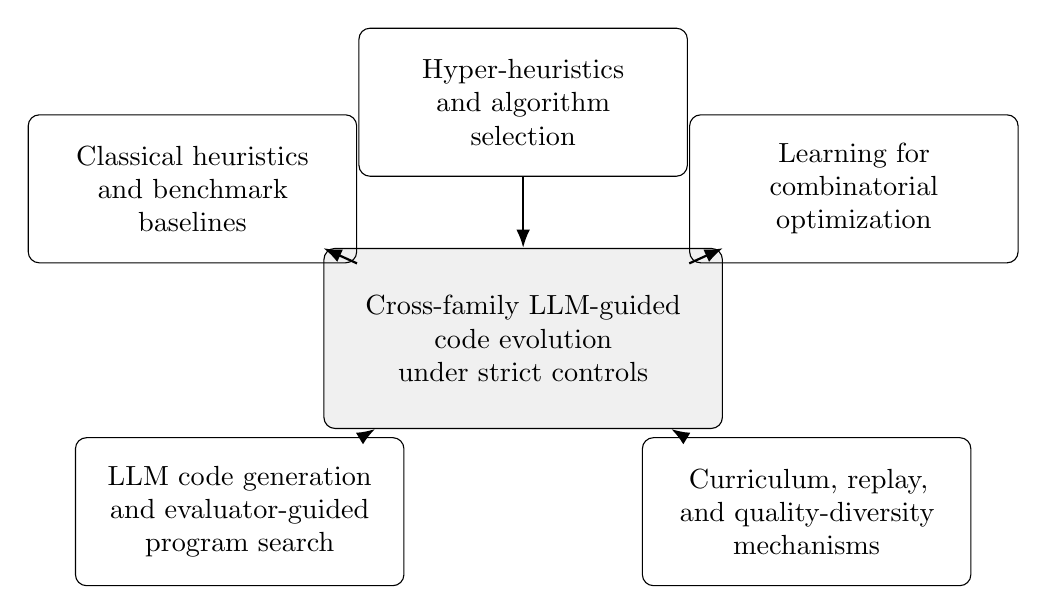
\begin{tikzpicture}[
  box/.style={draw, rounded corners, align=center, text width=1.55in, minimum height=0.74in},
  core/.style={draw, rounded corners, align=center, fill=black!6, text width=1.9in, minimum height=0.9in},
  line/.style={-Latex, thick}
]
\node[core] (core) at (0,0) {Cross-family LLM-guided\\code evolution\\under strict controls};
\node[box] (heur) at (-4.2,1.9) {Classical heuristics\\and benchmark\\baselines};
\node[box] (hyper) at (0,3.0) {Hyper-heuristics\\and algorithm\\selection};
\node[box] (mlco) at (4.2,1.9) {Learning for\\combinatorial\\optimization};
\node[box] (llm) at (-3.6,-2.2) {LLM code generation\\and evaluator-guided\\program search};
\node[box] (replay) at (3.6,-2.2) {Curriculum, replay,\\and quality-diversity\\mechanisms};
\draw[line] (heur) -- (core);
\draw[line] (hyper) -- (core);
\draw[line] (mlco) -- (core);
\draw[line] (llm) -- (core);
\draw[line] (replay) -- (core);
\end{tikzpicture}
\caption[Conceptual synthesis of research threads]{Conceptual synthesis of the research threads integrated by the dissertation. The gap is
not any single ingredient in isolation, but the absence of a cross-family, validator-aware account
of how these ingredients interact when the object of search is executable heuristic code.}
\label{fig:lit-synthesis-map}
\end{figure}

The literature reviewed above supports five observations that matter directly for this thesis.

\begin{enumerate}[leftmargin=2em]
\item Classical optimization already provides strong benchmark libraries and strong heuristic
baselines \cite{reinelt1991,lin1973,helsgaun2000,clarke1964,uchoa2017,vidal2022hgs}.
\item Hyper-heuristics and algorithm selection offer established ways to reason about search in
heuristic space rather than solution space \cite{rice1976,burke2013,dokeroglu2024}.
\item Modern code LLMs are strong enough to generate executable programs, especially when combined
with repeated sampling, testing, and repair
\cite{chen2021codex,austin2021program,li2022alphacode,jain2024livecodebench}.
\item Evaluator-guided algorithm discovery with AI is now credible, but existing success stories
often depend on specialized evaluators, narrow scopes, or problem formulations that differ from
full-program benchmark optimization
\cite{mankowitz2023alphadev,romeraparedes2024funsearch,liu2023lmea}.
\item Curriculum, replay, and diversity mechanisms are theoretically motivated, but their value in
LLM-guided \emph{code evolution} remains an empirical question rather than a settled fact
\cite{bengio2009curriculum,schaul2015prioritized,pugh2016qd}.
\end{enumerate}

The present thesis addresses a gap at the intersection of these points. There is still no clear
empirical account of how LLM-guided code evolution behaves across multiple benchmark families when
evaluated with replicated runs, strong classical baselines, replay alternatives, and strict
validator-based transfer tests. The dissertation therefore centers on a conservative cross-family
study of executable heuristics rather than on isolated positive examples.

\section{Chapter Summary}
\label{sec:lit-summary}

This chapter provided the technical context for the dissertation in four steps. It positioned the
work within algorithm selection and hyper-heuristics, where the central object of search is a
heuristic procedure rather than a single candidate solution. It reviewed the benchmark optimization
families that make the empirical claims meaningful, including the standard TSP, ATSP, and CVRP
formulations and their mature baseline literatures. It also situated the project within modern
code-generation and evaluator-guided program-search research, where LLMs are most credible when
paired with strong external verification. Finally, it showed why replay, curriculum, and diversity
mechanisms must be evaluated under careful experimental discipline rather than inferred from
isolated positive cases. The next chapter turns from that context to the experimental design used
to study the gap identified here.


\bibliographystyle{siam}
\bibliography{references}

\end{document}
